\documentclass[12pt]{article}

% double-spacing
\usepackage{setspace}
\doublespacing

%% line numbers
%% (turn on before submission)
%\usepackage{lineno}
%\linenumbers

% 1 inch margins
\usepackage[margin=1in]{geometry}

% text color
\usepackage{xcolor}

% bold symbols
\usepackage{bm}

% matrices
\usepackage{amsmath}

% images
\usepackage{graphicx}

% links
\usepackage{hyperref}

% highlight text that needs editing in red
\newcommand{\edit}[1]{{\color{red}{#1}}}
\newcommand{\add}[1]{{\color{red}{[... #1 ...]}}}

% bibliography
\usepackage[super]{natbib} % superscripts
\renewcommand{\refname}{} % empty title
\setcitestyle{citesep={,}} % comma separated

% add "S" before section numbers and figure numbers
\renewcommand{\thesection}{S\arabic{section}}
\renewcommand{\thesubsection}{S\arabic{subsection}}
\renewcommand{\thefigure}{S\arabic{figure}}

% add lists of figures and tables to TOC
\usepackage[nottoc]{tocbibind}

%\newcommand{\supplementarysection}{%
%  \setcounter{figure}{0}% Reset figure counter
%  \let\oldthefigure\thefigure% Capture figure numbering scheme
%  \renewcommand{\thefigure}{S\oldthefigure}% Prefix figure number with S
%  \section{Supplementary section}% Set supplementary section
%  %\let\oldchapter\chapter% Copy \chapter into \oldchapter
%  %\renewcommand{\chapter}{% Update \chapter
%  %  \let\thefigure\oldthefigure% Copy \thefigure into \oldthefigure
%   % \let\chapter\oldchapter% Restore original \chapter
%   % \oldchapter% Call original \chapter
%  %}
%}

% reference across files
\usepackage{xr}
\externaldocument{SpuriousAssociations}



%% title
\title{Supplemental Information}




\begin{document}

\maketitle
\tableofcontents % need to fix numbering

\newpage
\listoffigures

\newpage
%\listoftables

%\supplementarysection

\newpage
\section{PCs versus Model-Based Admixture Proportions}

In many African American populations, only one principal component may be needed to capture ancestral heterogeneity, at least with respect to differences in the relative proportion of African and European continental ancestry.
We investigated whether this statement holds true in three samples of African American individuals from the Women's Health Initiative SNP Health Association Resource (WHI SHARe) and two Trans-Omics for Precision Medicine (TOPMed) contributing studies: the Jackson Heart Study (JHS) and the Chronic Obstructive Pulmonary Disease Genetic Epidemiology Study (COPDGene).
Comparing model-based admixture proportions (estimated using \texttt{RFMix} \citep{rfmix} in WHI SHARe and an unsupervised \texttt{ADMIXTURE} \citep{admixture} analysis in JHS and COPDGene) to principal components shows that the first PC is in fact highly correlated with the inferred proportion of African ancestry in these samples, while later PCs show very little correlation with genome-wide continental ancestry.
This pattern holds regardless of whether PCs are generated with (Figure \ref{fig:prunedpcsvsglob}) or without (Figure \ref{fig:pcsvsglob}) prior filtering or pruning based on linkage disequilibrium (LD).

\begin{figure}[!htb]
\center
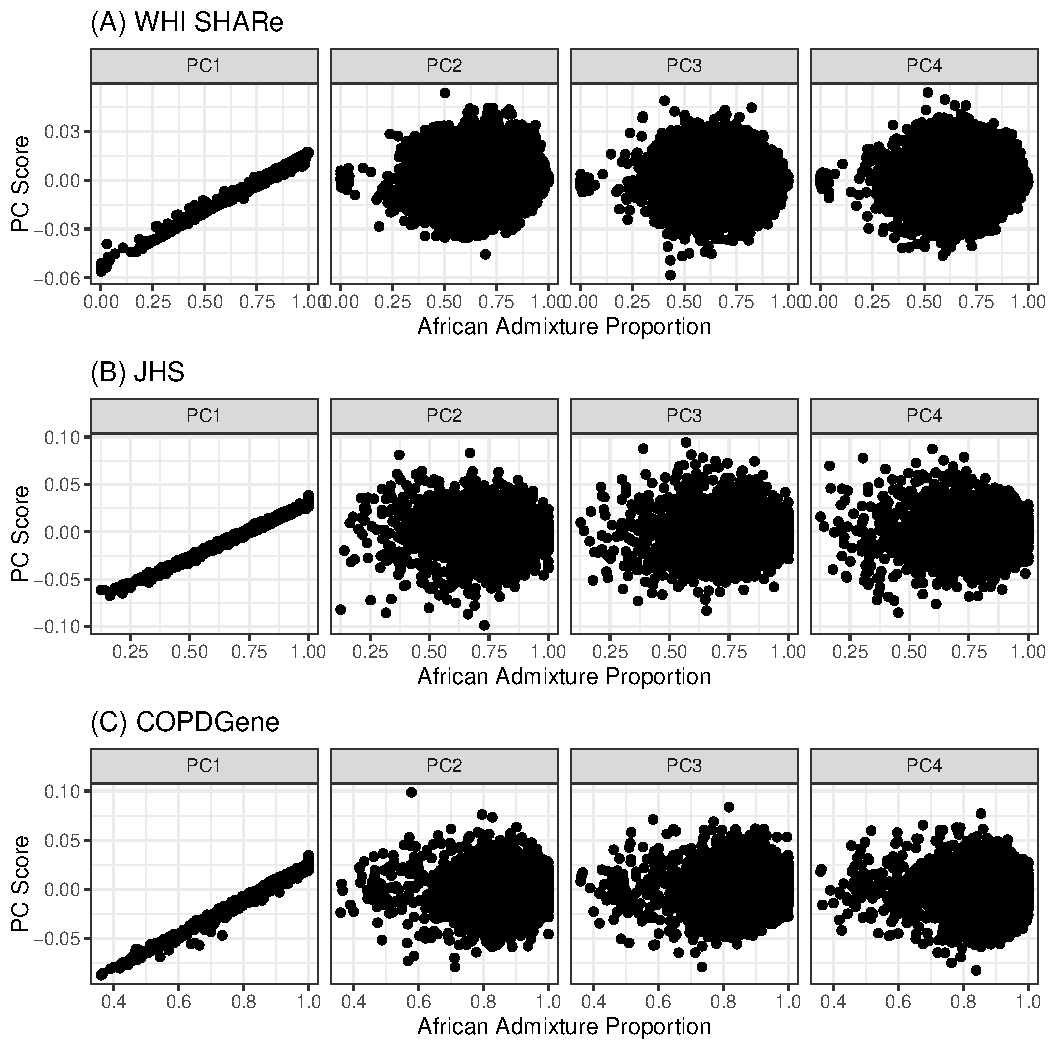
\includegraphics[width=\textwidth]{figs/pcs_vs_global/pcs_vs_global}
\caption{Scatterplots of estimated African admixture proportions versus the first four PCs in (A) WHI SHARe, (B) TOPMed JHS, and (C) TOPMed COPDGene African Americans. Here we consider PCs that were generated without any prior LD-based filtering or pruning.}
\label{fig:pcsvsglob}
\end{figure}

\begin{figure}[!htb]
\center
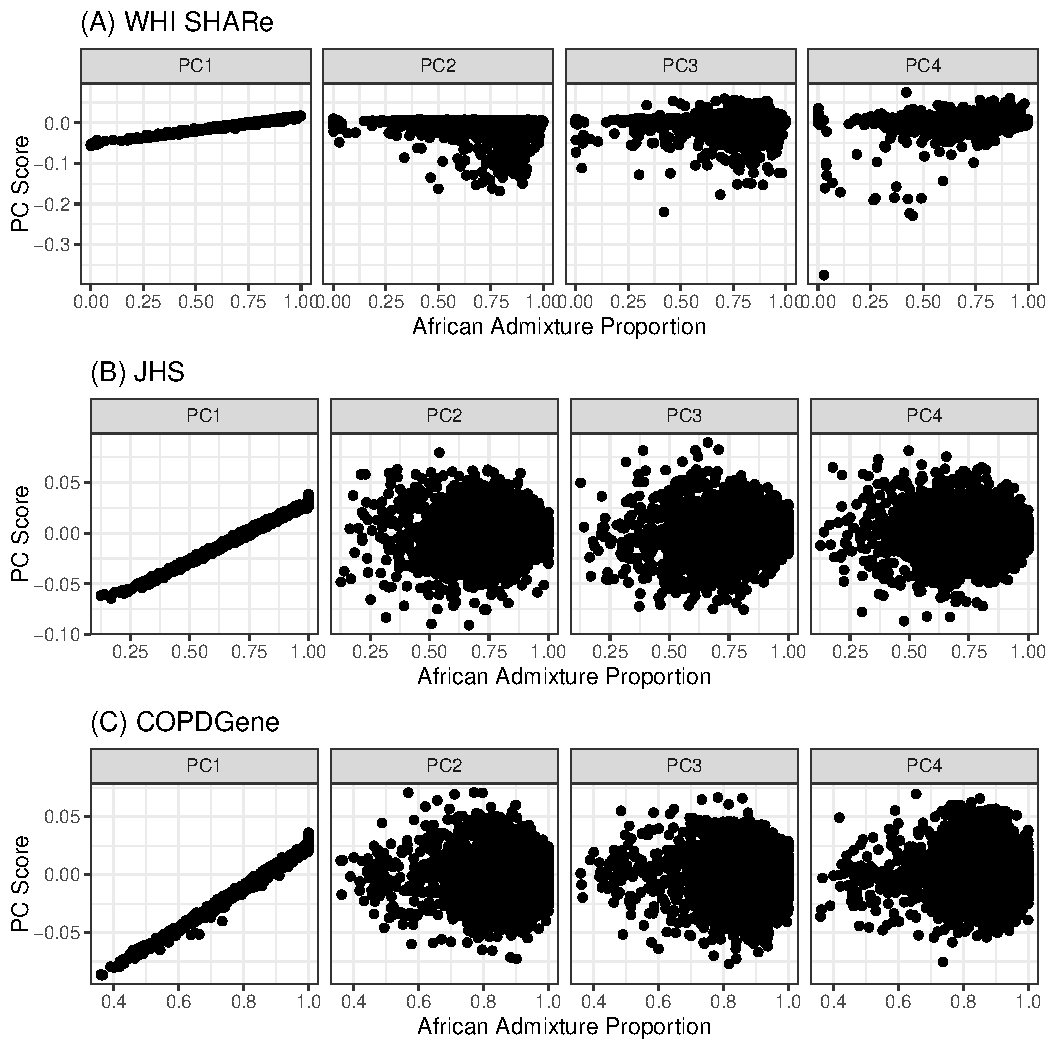
\includegraphics[width=0.9\textwidth]{figs/pcs_vs_global/pruned_pcs_vs_global}
\caption{Scatterplots of estimated African admixture proportions versus the first four PCs in (A) WHI SHARe, (B) TOPMed JHS, and (C) TOPMed COPDGene African Americans. Here we consider PCs that were generated after both LD pruning ($r^2 = 0.1$, window size = 0.5 Mb) and filtering previously identified high-LD regions (Table \ref{tab:highLD}).}
\label{fig:prunedpcsvsglob}
\end{figure}




\section{Comparison of PCA Pre-Processing Choices}

We have shown that adjusting for principal components that capture small regions of the genome rather than genome-wide ancestry can induce spurious associations in genome-wide association studies.
This problematic behavior occurred in our analysis of genotype data from WHI SHARe African Americans when PCs were generated using all 551,025 available SNPs or if we excluded regions identified in the literature as being potentially problematic for PCA (Table \ref{tab:highLD}).
However, problems were ameliorated when we used PCs that were generated after strict LD pruning, using an $r^2$ threshold of 0.1 and window size of 0.5 Mb.
In this section, we further investigate the behavior of PCs generated after different filtering techniques.

Many authors have suggested using an $r^2$ threshold of 0.2 for LD pruning prior to running PCA \edit{\citep{142, 68, 164, 136, 135, 131, 66, 129}}.
Furthermore, this threshold is the default for LD pruning software such as \texttt{SNPRelate} \citep{snprelate}.
However, in our analysis of WHI SHARe data, we found that using an $r^2$ threshold of 0.2 prior to running PCA still led to one of the top PCs (the fourth) being highly correlated with small regions of the genome, while if we used a stricter threshold of 0.1 the peaks have disappeared (at least for the top four PCs).
See Figure \ref{fig:corr-compare-prune} for a comparison of the correlation between PCs and genotypes in WHI SHARe African Americans across different choices of $r^2$ threshold.

When performing LD pruning, another choice that practitioners have to make is the window size. 
In the literature, various window sizes have been suggested, including 10 Mb \edit{\citep{89}}, 2 Mb \edit{\citep{68}}, or 0.5 Mb (the \texttt{SNPRelate} default, and others have suggested that window size may not have a big impact \edit{\citep{136}}.
In our analysis of WHI SHARe data, we see little difference in the correlation between PCs and genotypes across different choices of window sizes: see Figure \ref{fig:corr-compare-window}.
Smaller window size are less computationally intensive, so we used the window size of 0.5 Mb for the remainder of our analyses.

Finally, we also considered filtering out regions that were highly correlated with PCs in our own data, as has been done previously \edit{\citep{66, 142}}.
To implement this data-based filtering, we investigated the SNP loadings for each of the top four PCs. 
Starting with the second PC, we found the SNP on each chromosome with the largest loading: if this loading was larger than 0.005, we excluded the SNP and all SNPS within $M$ Mb; if the loading was small, we kept all SNPs on the chromosome.
(We considered $M = 1, 5, 10$, and $20$ Mb.) 
We repeated this process for PCs 3 and 4, then re-ran PCA using the remaining SNPs.
Using these new PCs, we re-calculated SNP loadings and looked to see if there were still regions of the genome that were driving the PCs.
If so, we repeated the entire process.
This data-based filtering process is very tedious, and even after four rounds of exclusions with $M = 5$ Mb we found that the problematic behavior did not totally go away (Figure \ref{fig:corr-compare-exclude}).

In WHI SHARe data, at least, strict LD pruning is the most effective of the pre-processing steps that we considered in eliminating the correlation between PCs and genotypes in small regions of the genome.

\begin{figure}[!htb]
\center
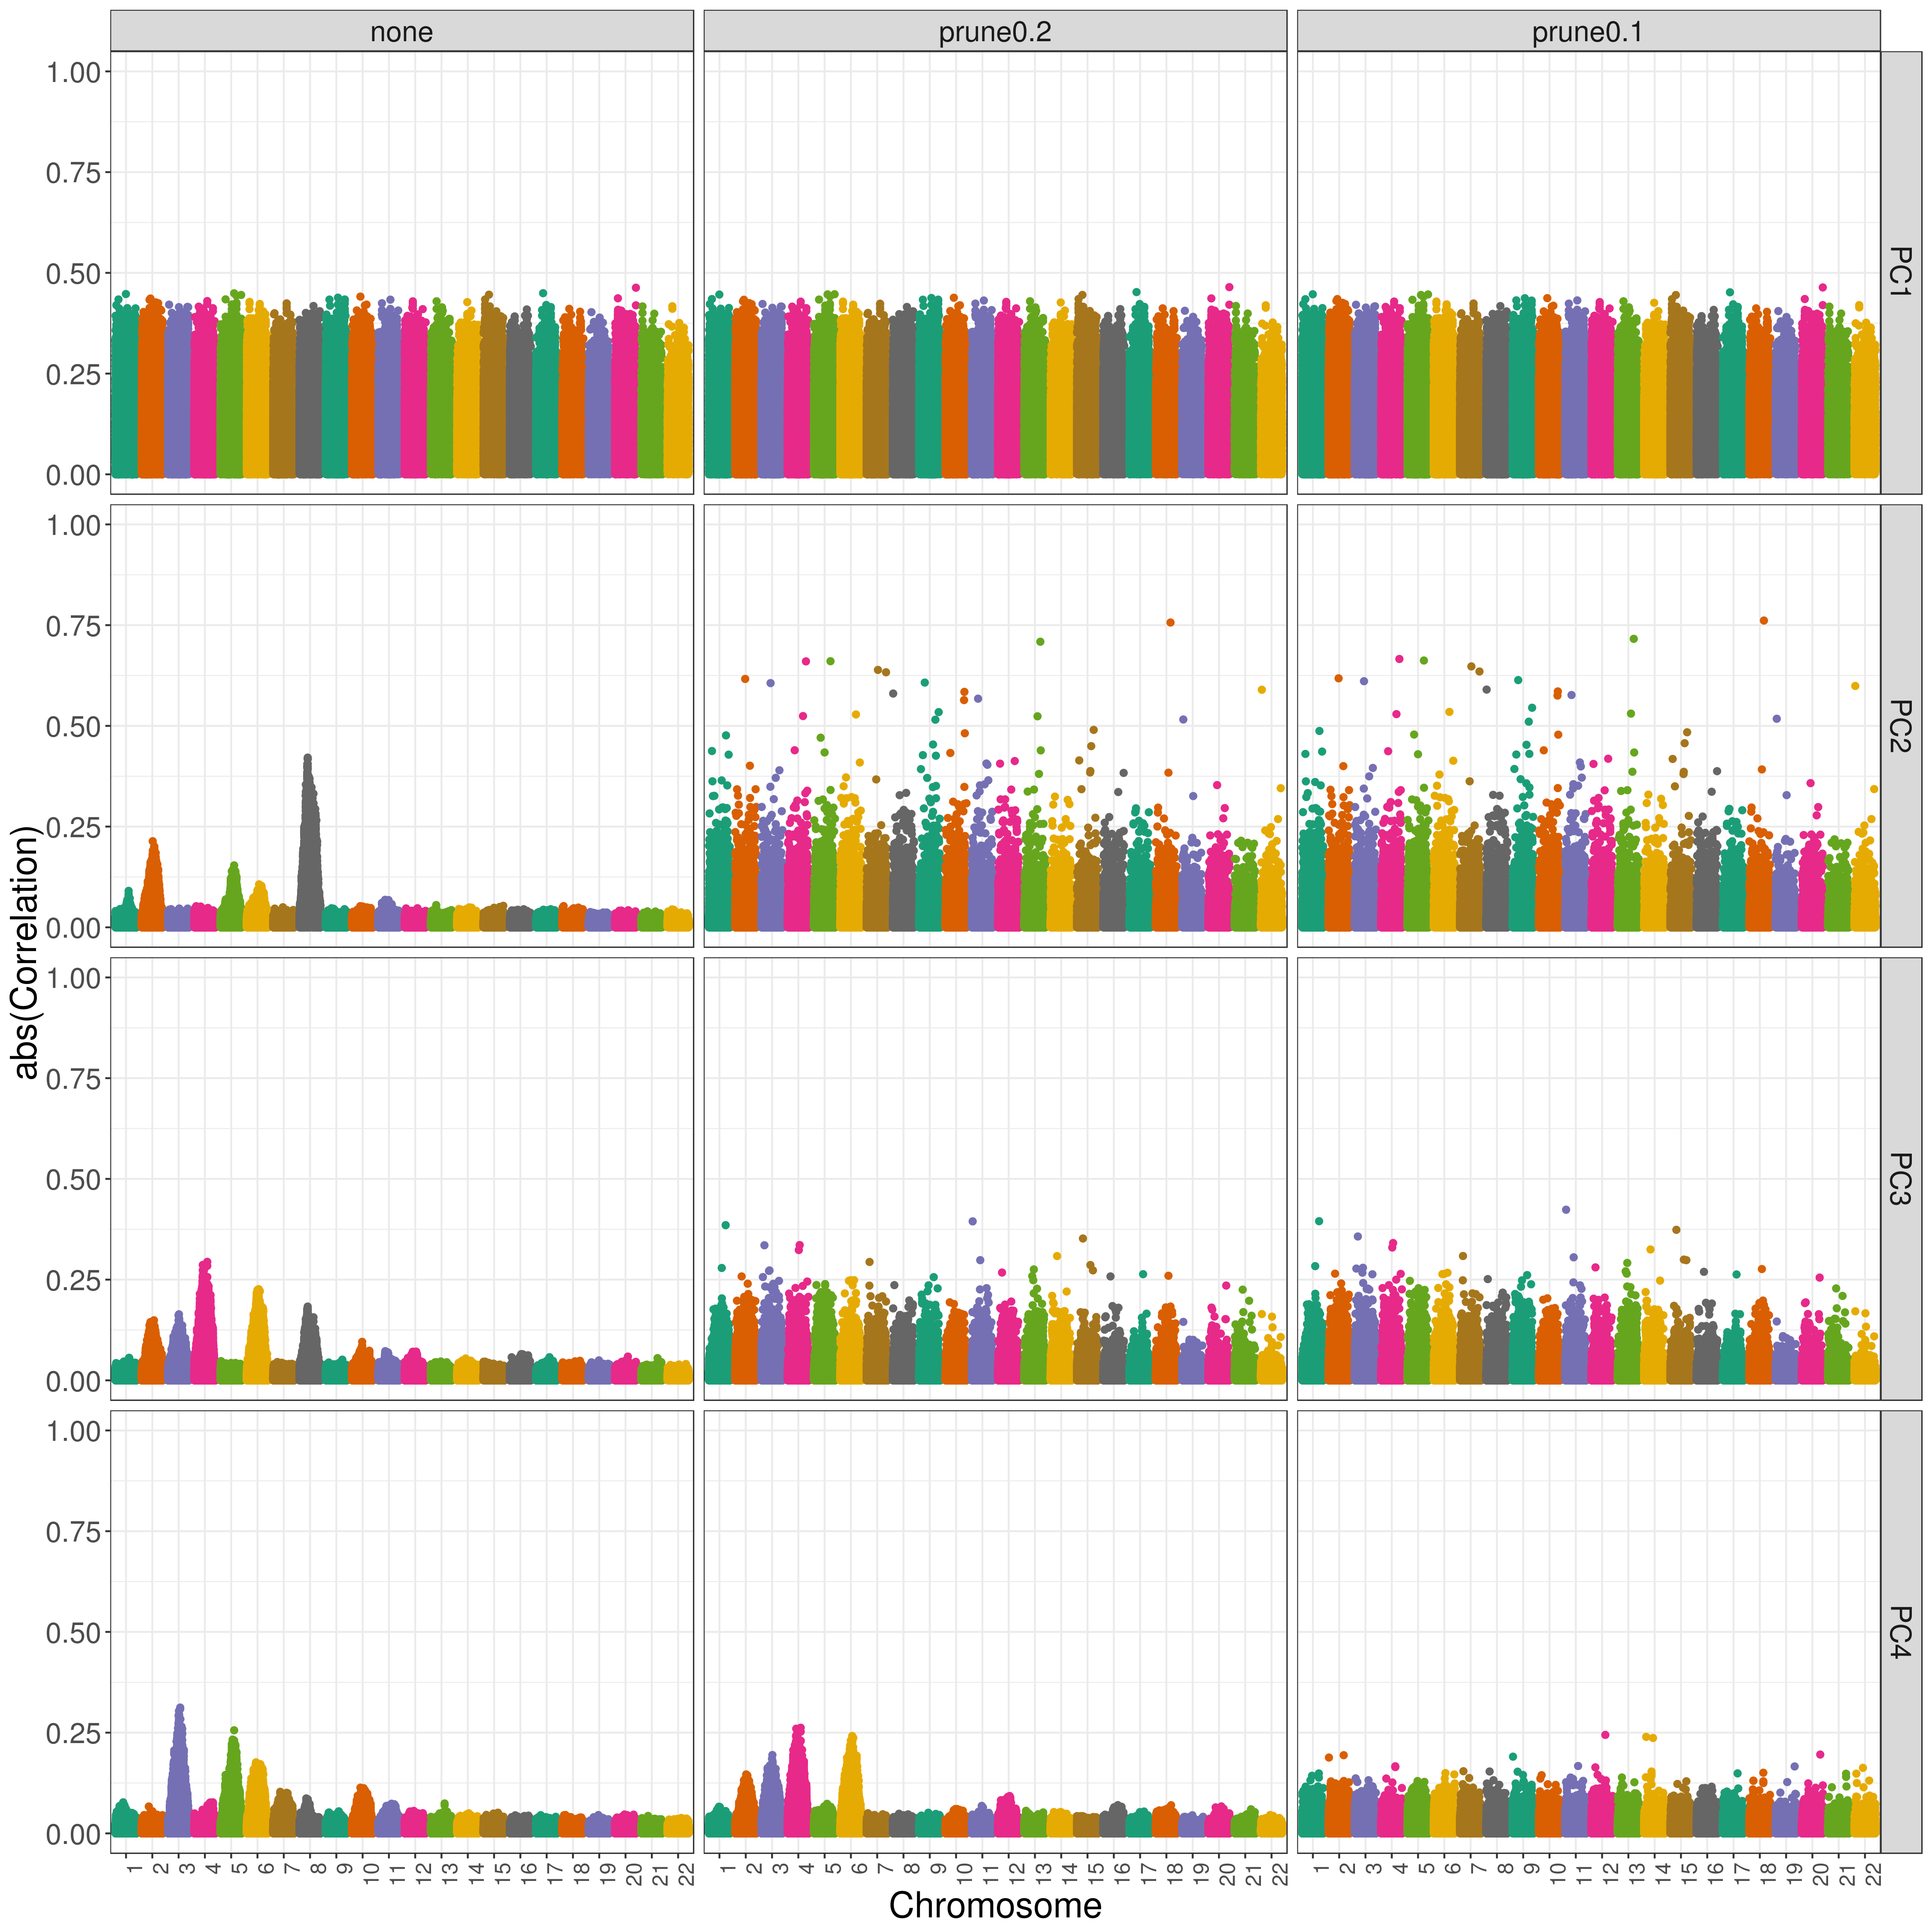
\includegraphics[width=\textwidth]{figs/pc_geno_corr/pc_geno_corr_compare_prune}
\caption{Correlation between PCs and genotypes in WHI SHARe African Americans using different LD pruning thresholds. Each panel plots the absolute value (abs) of the correlation between principal components and genotypes on the y-axis versus the position along the genome on the x-axis.  Panels are organized vertically according to which PC is being investigated (1, 2, 3, 4) and horizontally according to what $r^2$ threshold was used when running LD pruning prior to PCA (\textit{none}: no LD pruning, \textit{prune0.2}: LD pruning with an $r^2$ threshold of 0.2 and window size of 0.5 Mb, and \textit{prune0.1}: LD pruning with an $r^2$ threshold of 0.1 and window size of 0.5 Mb).}
\label{fig:corr-compare-prune}
\end{figure}

\begin{figure}[!htb]
\center
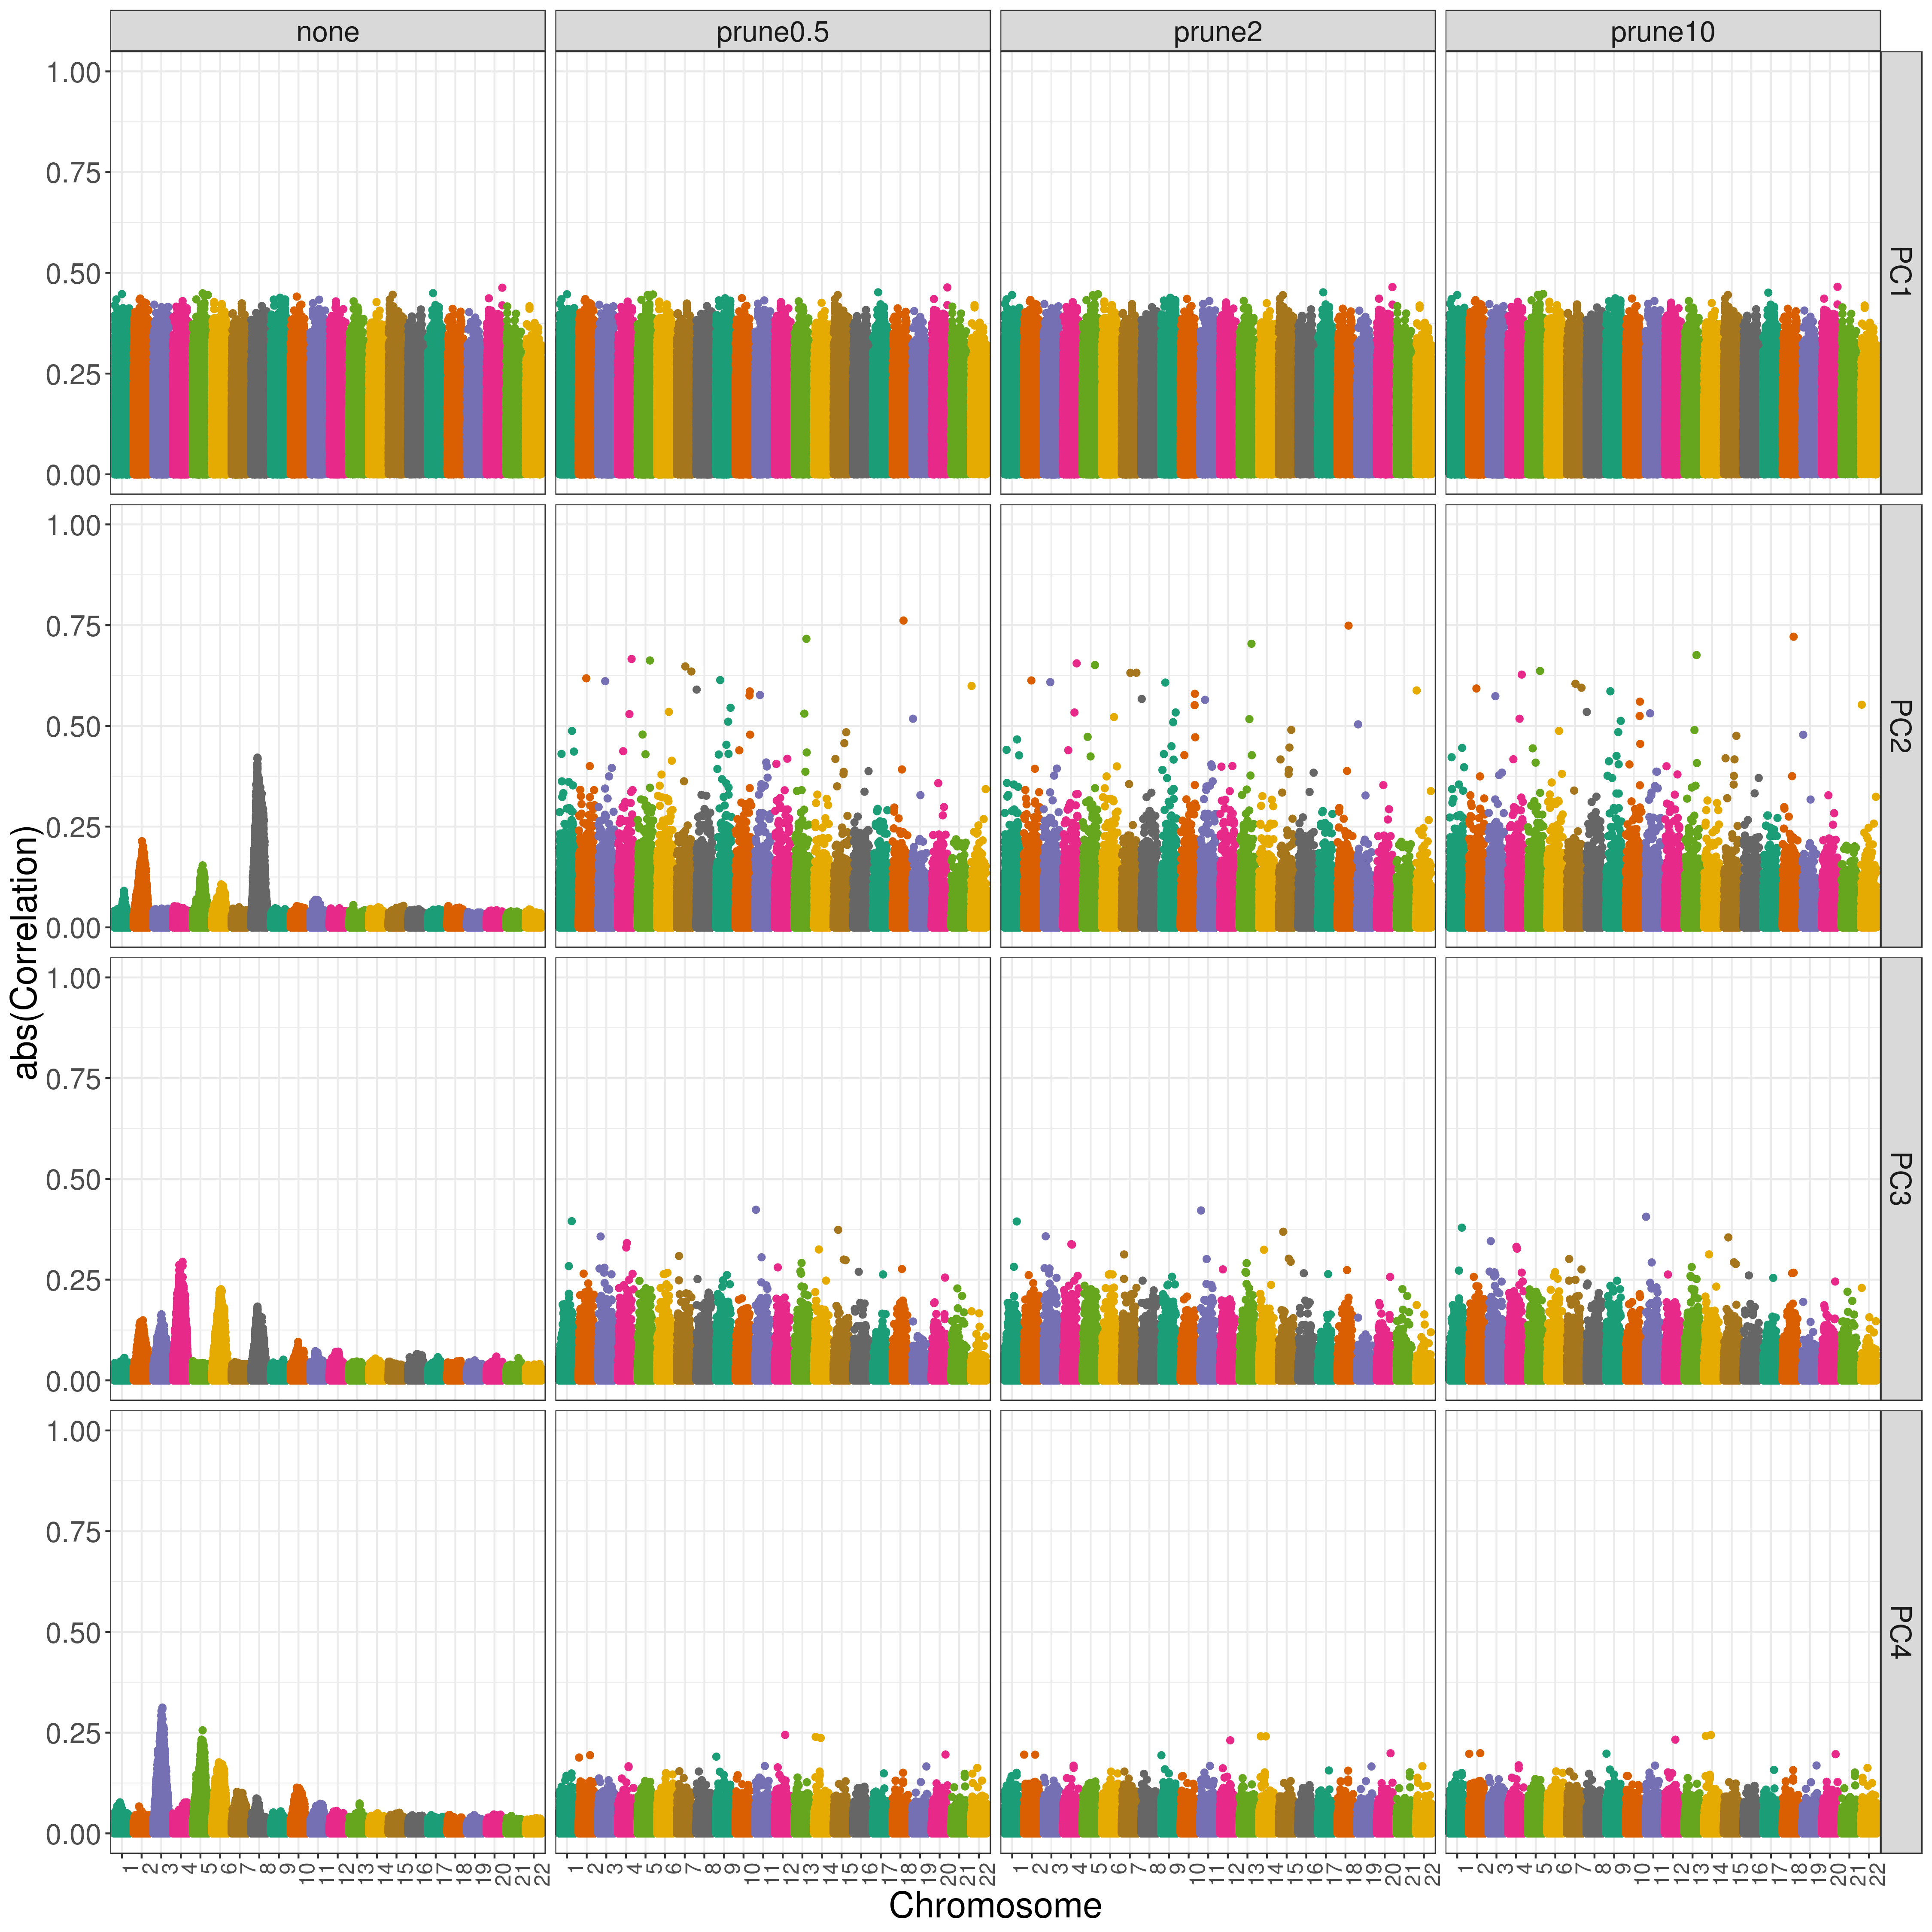
\includegraphics[width=\textwidth]{figs/pc_geno_corr/pc_geno_corr_compare_window}
\caption{Correlation between PCs and genotypes in WHI SHARe African Americans using different LD pruning window sizes. Each panel plots the absolute value (abs) of the correlation between principal components and genotypes on the y-axis versus the position along the genome on the x-axis.  Panels are organized vertically according to which PC is being investigated (1, 2, 3, 4) and horizontally according to what window size was used when running LD pruning prior to PCA (\textit{none}: no LD pruning, \textit{prune0.5}: LD pruning with an $r^2$ threshold of 0.1 and window size of 0.5 Mb, \textit{prune2}: LD pruning with an $r^2$ threshold of 0.1 and window size of 2 Mb, and \textit{prune10}: LD pruning with an $r^2$ threshold of 0.1 and window size of 10 Mb).}
\label{fig:corr-compare-window}
\end{figure}

\begin{figure}[!htb]
\center
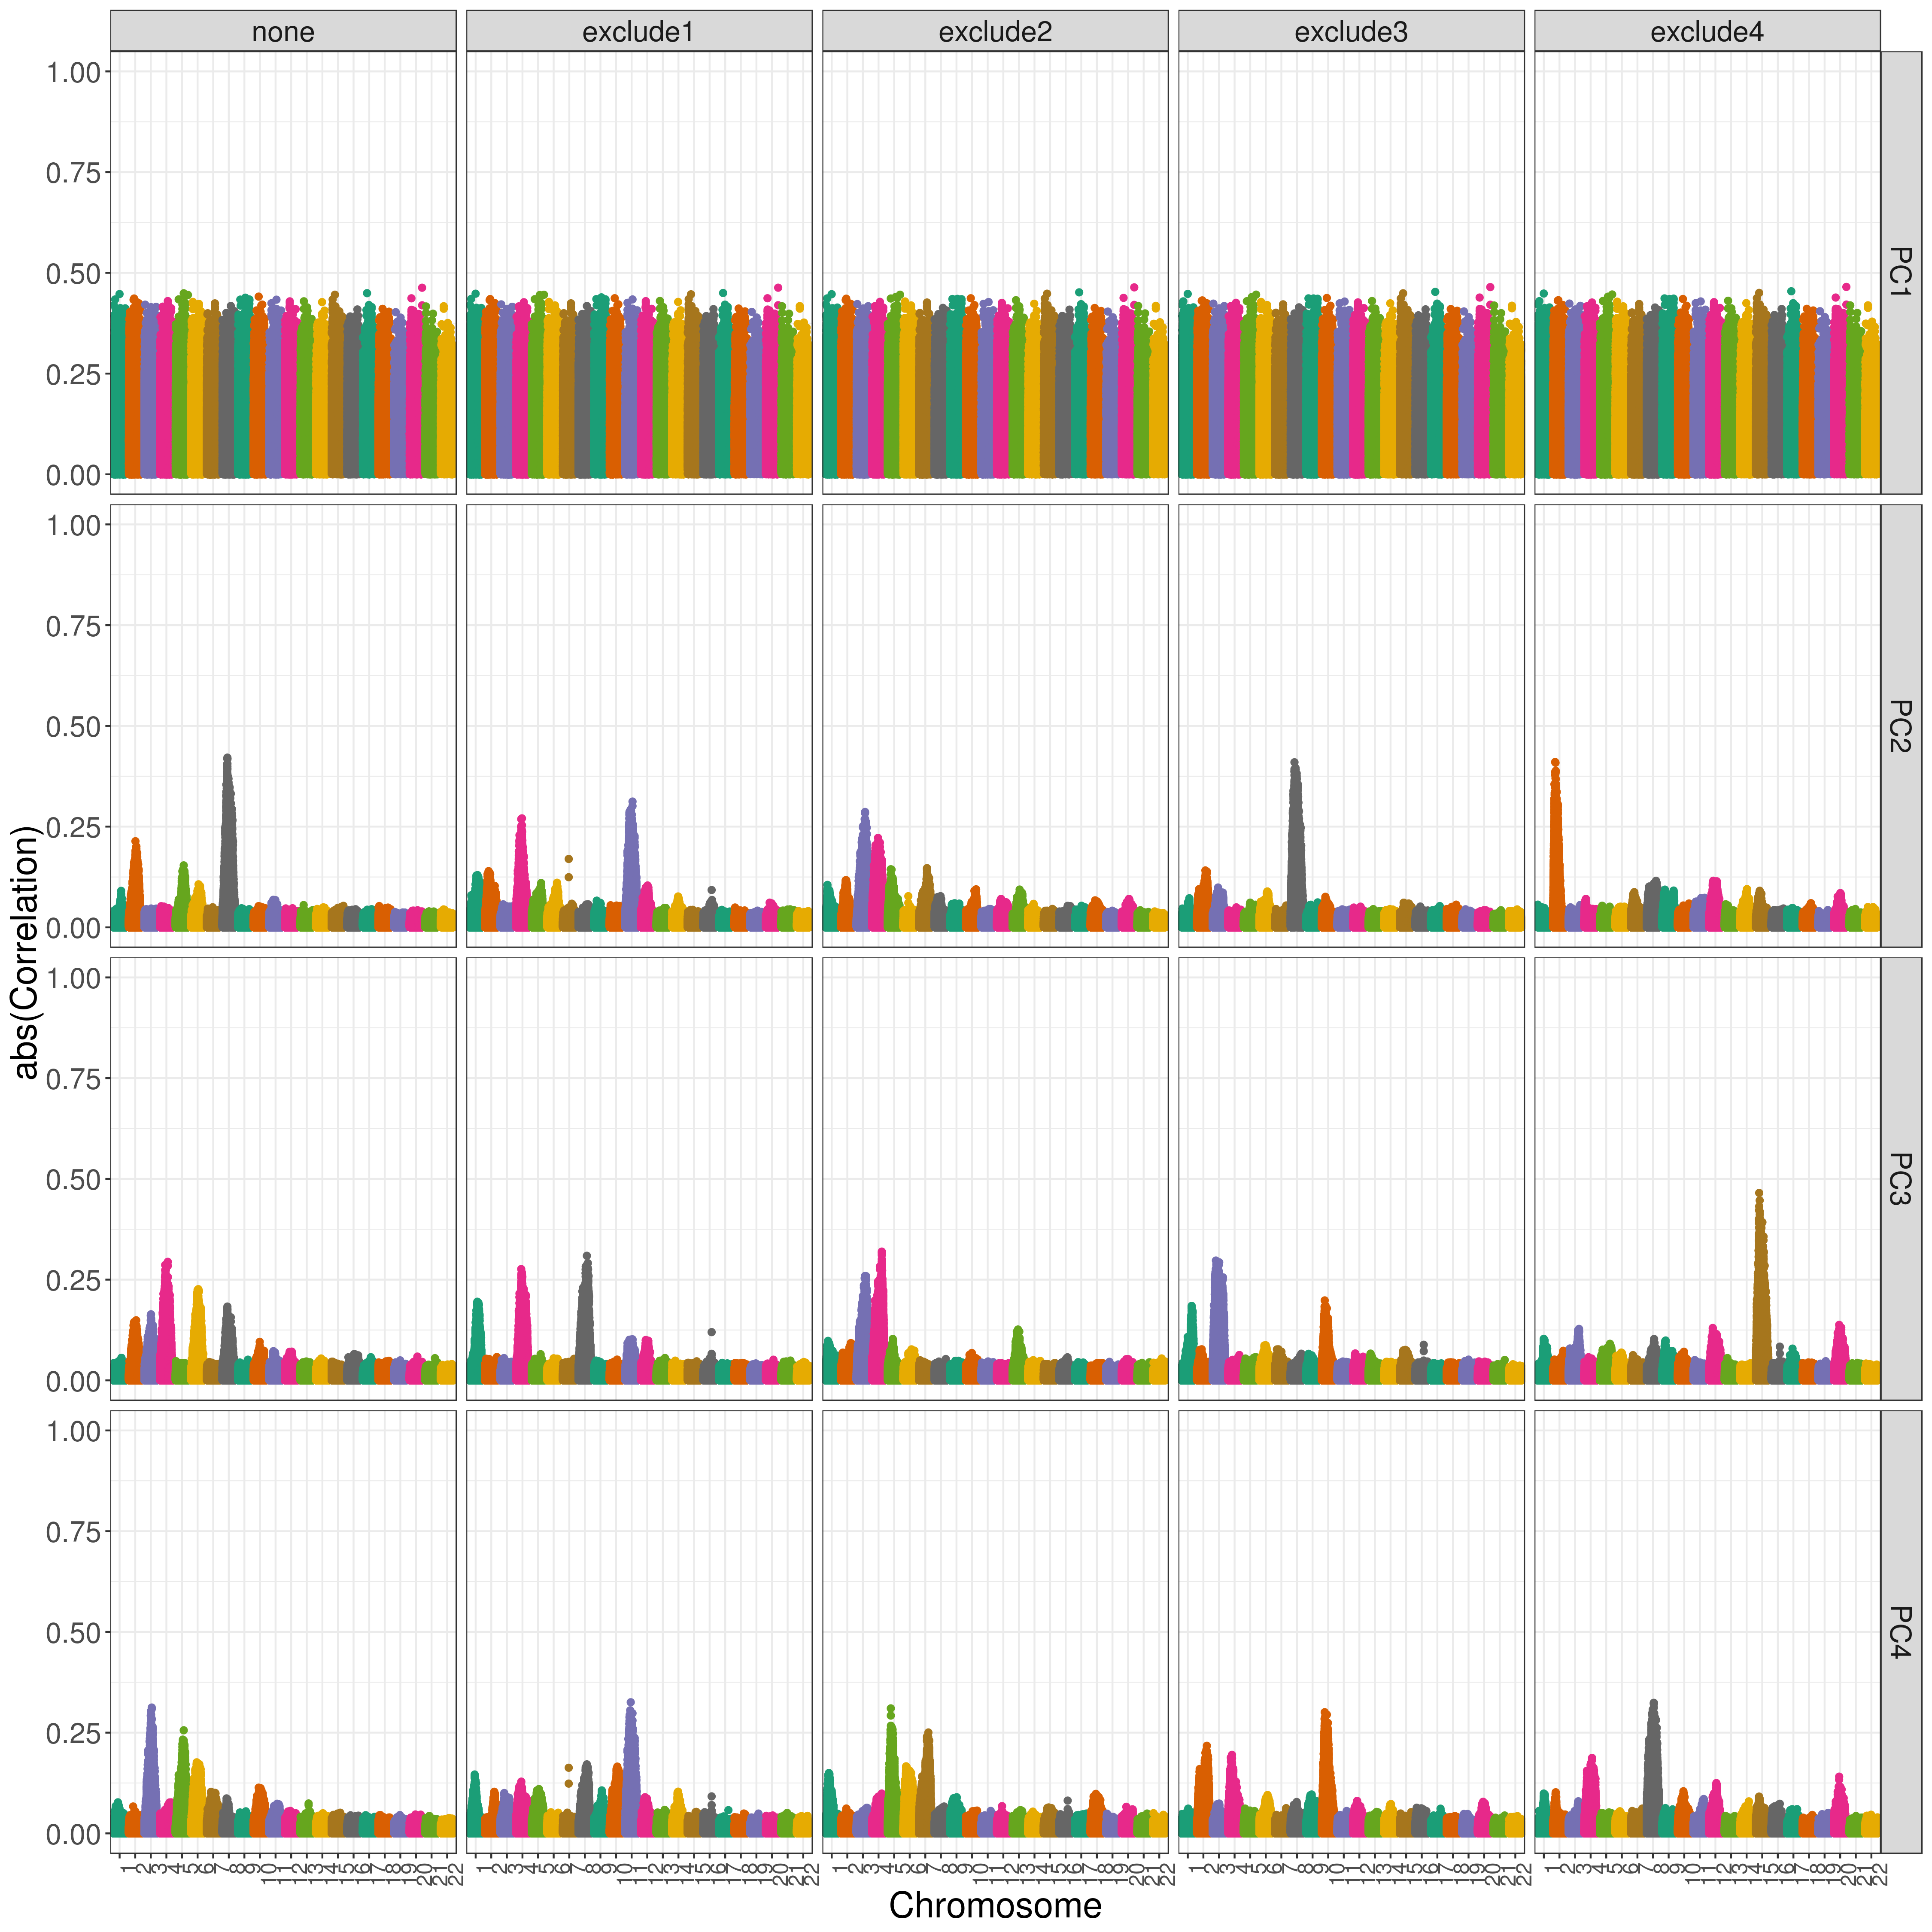
\includegraphics[width=\textwidth]{figs/pc_geno_corr/pc_geno_corr_compare_exclude}
\caption{Correlation between PCs and genotypes in WHI SHARe African Americans after multiple rounds of data-based exclusions. Each panel plots the absolute value (abs) of the correlation between principal components and genotypes on the y-axis versus the position along the genome on the x-axis.  Panels are organized vertically according to which PC is being investigated (1, 2, 3, 4) and horizontally according to the number of iterations of our procedure for excluding regions highly correlated with PCs that were implemented prior to PCA (\textit{none}: no exclusions, \textit{exclude1}: one round of exclusions, \textit{exclude2}: two rounds of exclusions, etc.).}
\label{fig:corr-compare-exclude}
\end{figure}



\newpage
\section{Investigating PCs in a European American Population}

We have shown that principal components can capture multiple local genomic features, rather than genome-wide ancestry, unless careful pre-processing is performed prior to running PCA.
This observation is not entirely novel, but note that the patterns we observe in WHI SHARe, JHS, and COPDGene African Americans differ slightly from what has previously been observed in European populations.
In particular, in European populations a principal component might capture variation on a single chromosome \edit{add citations} whereas in these admixed populations we see PCs driven by contributions from variants across several chromosomes.
Although the focus of our work has been on admixed individuals, we were also able to run PCA on a sample of individuals with European ancestry using the COPDGene European Americans that we had excluded from our primary analyses. 
In this sample, we see patterns similar to those observed by previous authors, with the second and third principal components driven primarily by variants on a single chromosome: chromosome 11 (Figure \ref{fig:corr-Eur}).
This difference in what is captured by principal components in European populations versus admixed populations (i.e., variants on one chromosome versus multiple) has important implications: only when a PC captures \textit{multiple} local genomic features does the possibility of collider bias arise.
Thus, particular care must be taken when performing genome-wide association studies in admixed populations to ensure that models to do not adjust for principal components that are highly correlated with variants on distinct chromosomes.

\begin{figure}[!htb]
\center
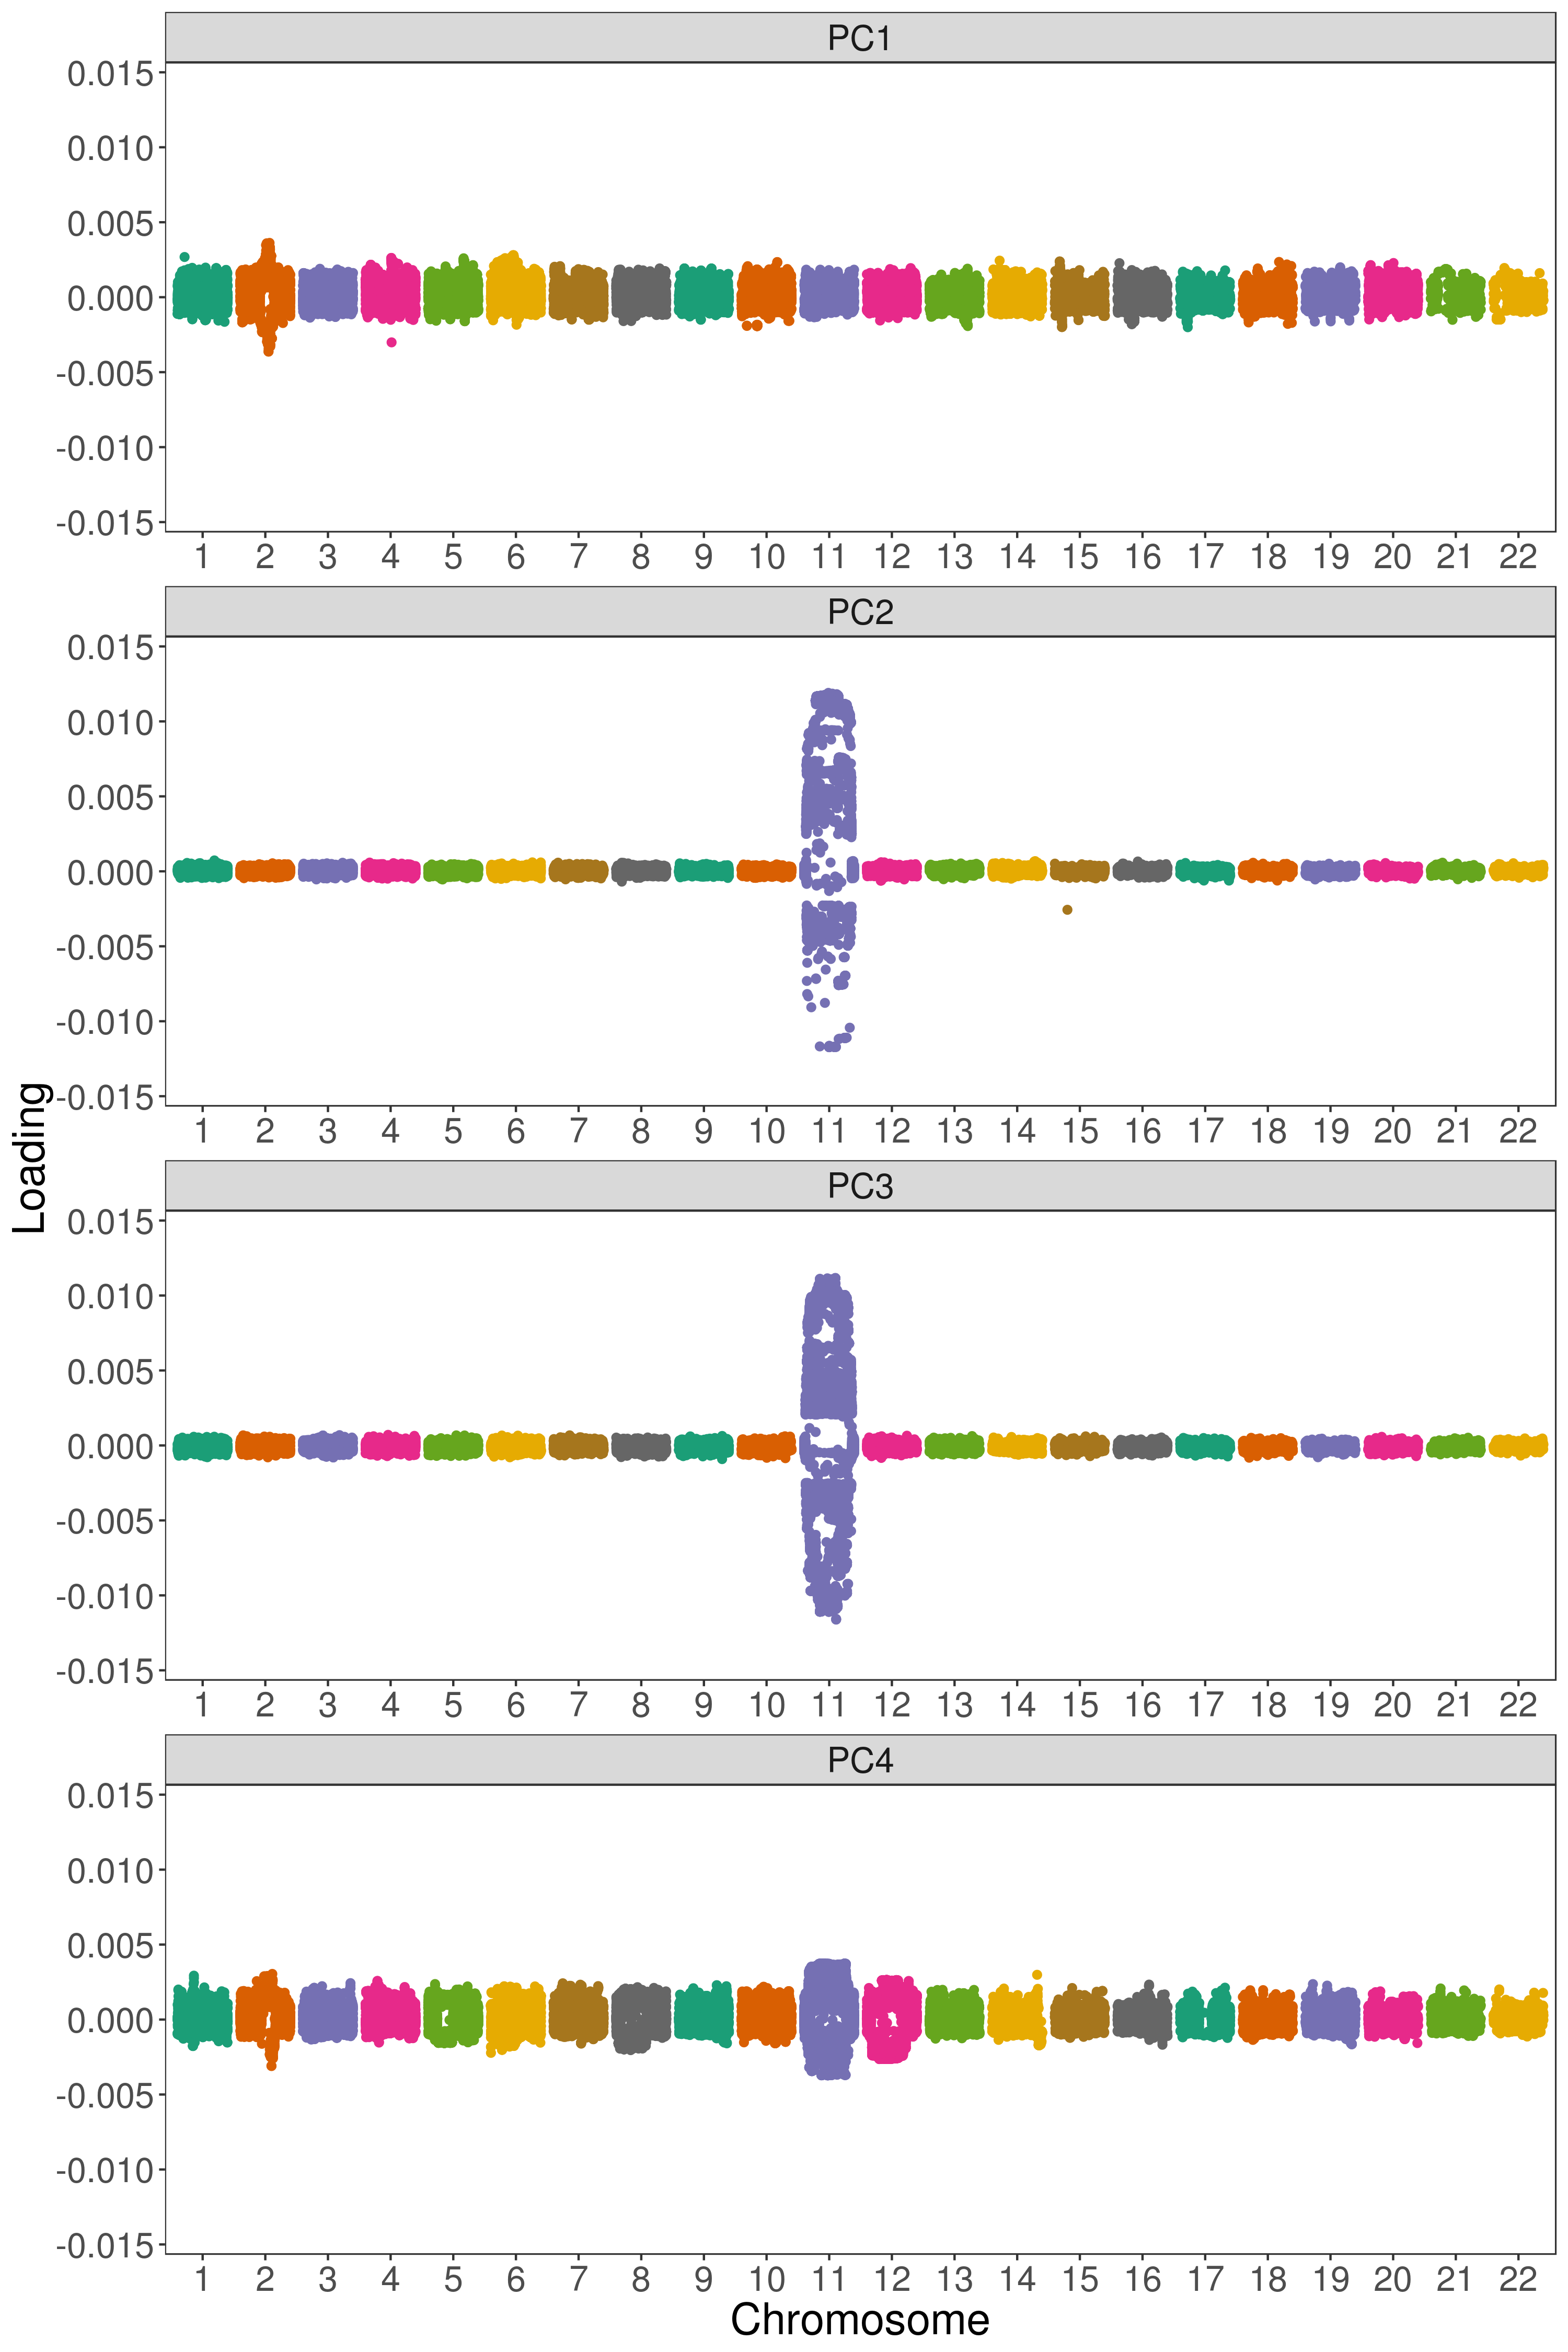
\includegraphics[width=0.8\textwidth]{figs/COPD/EUR_prune_FALSE_1_0_0.01_snprelate_load_1}
\caption{SNP loadings for naively generated PCs in COPDGene European Americans. Each panel plots the principal component loading (y-axis) versus the position along the genome (x-axis) for each variant. Panels are organized vertically according to which PC is being investigated (1, 2, 3, 4). Unlike in admixed populations, we see a single peak on chromosome 11.}
\label{fig:corr-Eur}
\end{figure}


\newpage
\section{Theoretical Results}

In the Results section, above, we present the expected effect size estimates for GWAS models using different techniques for adjusting for ancestral heterogeneity: see Equations \ref{eqn:collider}, \ref{eqn:unadjusted}, \edit{add reference number for third equation}.
In this Appendix, we provide details and simulation studies validating these theoretical results.

\subsection{The assumed data-generating mechanism}

We consider an admixed population with two ancestral populations, $n$ individuals, and admixture proportions $\boldsymbol{\pi}_i = \begin{pmatrix} \pi_{i} & 1-\pi_{i} \end{pmatrix}^\top$ that are allowed to vary across the population. 
We refer to the two ancestral populations as \textit{Ancestral Population 1} and \textit{Ancestral Population 2}, with $\pi_i$ representing the genome-wide proportion of genetic material inherited by individual $i$ from Ancestral Population 1 and $1-\pi_i$ representing the proportion of genetic material inherited from Ancestral Population 2. 
We denote local ancestry by $\mathbf{a}_{ij} = \begin{pmatrix} a_{ij} & 2 - a_{ij} \end{pmatrix}^\top,$ where $a_{ij}$ and $2-a_{ij}$ are the number of alleles inherited by individual $i$ from Ancestral Populations 1 and 2, respectively, at locus $j$.
Genotypes, quantified as the number of copies of some pre-specified allele carried by individual $i$ at locus $j$, are represented by $g_{ij}$.
We consider two \textit{unlinked} loci $j = 1, 2$ (e.g., loci on distinct chromosomes) and assume that data are generated according to the following hierarchical model: 
\begin{align*}
\pi_i &\overset{\text{i.i.d.}}{\sim} F \text{ for some distribution } F\\
a_{ij} \mid \pi_i &\overset{\text{i.i.d}}{\sim} \text{Binomial}(2, \pi_i), \ j = 1, 2\\
g_{ij} \mid a_{ij}, \mathbf{p}_j &\overset{\text{ind.}}{\sim} \text{Binomial}(a_{ij}, p_{j1}) + \text{Binomial}(2-a_{ij}, p_{j2}), \ j = 1, 2 
\end{align*}
where $p_{j1}, p_{j2}$ are allele frequencies at locus $j$ in Ancestral Populations 1 and 2, respectively. Note that since the two loci under consideration are unlinked, we assume that local ancestry and genotypes at these loci are conditionally independent.

We assume that our quantitative trait of interest $\mathbf{y}$ depends only on the genotype at locus 1 ($j = 1$), and we allow for the possibility that the admixture proportions $\boldsymbol\pi$ have a direct effect on the trait (e.g., through environmental differences across ancestral populations). More specifically, we assume that this trait is generated according to $$y_i  = \beta_0 + \beta_1 g_{i1} + \beta_\pi \pi_i + \epsilon_i, \ \ \epsilon_i \overset{\text{i.i.d}}{\sim} (0, \sigma_\epsilon^2).$$
We refer to $\beta_1$ and $\beta_2$ as the true \textit{effect sizes} of loci 1 and 2, respectively. Since the trait only depends on the genotype at locus 1, the true effect size of locus 2 is $\beta_2 = 0$.
%We are interested in using genome-wide association studies (GWAS) and admixture mapping studies to investigate the association between loci 1 and 2 and the trait of interest. 

Assuming that data are generated according to the above-described mechanisms, and defining $E_\pi := E(\pi)$ and $V_\pi :=   \text{Var}(\pi)$, then the following statements are true:

\begin{itemize}
%\item $E[\pi] := E_\pi$
%\item $V[\pi] := V_\pi$
\item $E(a_j) = 2E_\pi, \ j = 1, 2$
\item $V(a_j) = 2\{V_\pi + E_\pi(1-E_\pi)\}, \ j = 1, 2$
\item $\text{Cov}(a_1, a_2) = 4V_\pi$
\item $\text{Cov}(a_j, \pi) = 2V_\pi, \ j = 1, 2$
\item $E(g_j) = 2\{p_{j2} + (p_{j1}-p_{j2})E_\pi\}, \ j = 1, 2$
\item $V(g_j) = 2[p_{j2}(1-p_{j2}) + (p_{j1}-p_{j2})(1-p_{j1}-p_{j2})E_\pi + (p_{j1}-p_{j2})^2\{V_\pi + E_\pi(1-E_\pi)\}], \ j = 1, 2$
\item $\text{Cov}(g_1, g_2) = 4(p_{11}-p_{12})(p_{21}-p_{22})V_\pi$
\item $\text{Cov}(g_j, g_j) = 2(p_{j1}-p_{j2})\{V_\pi + E_\pi(1-E\pi)\}, \ j = 1, 2$
\item $\text{Cov}(g_j, g_k) = 4(p_{j1}-p_{j2})V_\pi, \ j \neq k$
\item $\text{Cov}(g_j, \pi) = 2(p_{j1}-p_{j2})V_\pi, \ j = 1, 2$
\end{itemize}

Furthermore, suppose we define a random variable %$z_a = g(a_1,a_2) + e, \ e \sim (\mu_e, \sigma_e^2)$ and 
$z_g = h(g_1, g_2) + e, \ e \sim (\mu_e, \sigma_e^2)$ for some function $h$. Then:
\begin{itemize}
%\item $E(z_a) = \mu_e + E\{g(a_1, a_2)\}$
%\item $V(z_a) = \sigma_e^2 + V\{g(a_1, a_2)\}$
%\item $\text{Cov}(\pi, z_a) = \text{Cov}[\pi, E\{g(a_1,a_2) \mid \pi\}]$
%\item $\text{Cov}(a_j, z_a) = 2\text{Cov}(\pi, z_a) + E[\text{Cov}\{a_j, g(a_1,a_2) \mid \pi\}], \ j = 1, 2$
%\item  $\text{Cov}(x_j, z_a) = (p_{j1}-p_{j2})\text{Cov}(a_j, z_a)  = (p_{j1}-p_{j2}) ( 2\text{Cov}(\pi, z_a) + E[\text{Cov}\{a_j, g(a_1,a_2) \mid \pi\}])\\ =  2(p_{j1}-p_{j2})\text{Cov}(\pi, z_a) + E\{\text{Cov}[x_j, g(a_1,a_2) \mid \pi \}], \ j = 1, 2$
\item $E(z_g) = \mu_e + E\{h(g_1, g_2)\}$
\item $V(z_g) = \sigma_e^2 + V\{h(g_1, g_2)\}$
\item $\text{Cov}(\pi, z_g) = \text{Cov}[\pi, E\{h(g_1,g_2) \mid \pi\}]$ 
\item  $\text{Cov}(a_j, z_g) = 2\text{Cov}(\pi, z_g) + E[\text{Cov}\{a_j, h(g_1,g_2) \mid \pi\}], \ j = 1, 2$
\item $\text{Cov}(g_j, z_g) = 2(p_{j1}-p_{j2}) \text{Cov}(\pi, z_x) + E[\text{Cov}\{g_j, h(g_1,g_2) \mid \pi\}], \ j = 1,2$
\end{itemize}

These results are straightforward to derive, using our assumed hierarchical data-generating model and the laws of total expectation $$E[x] = E\{E[x\mid y]\},$$ total variance $$V[x] = V\{E[x\mid y]\} + E\{ V[x \mid y] \},$$ and total covariance $$\text{Cov}[x,y] = \text{Cov}\{E[x\mid z], E[y\mid z]\} + E\{ \text{Cov}[x,y \mid z] \}.$$

\subsection{Expected effect size estimates}

\subsubsection{Unadjusted model}

\subsubsection{Admixture proportion adjusted model}

\subsubsection{Principal component adjusted model}


\subsection{Two locus simulations}

\edit{pull from dissertation}

\subsection{Whole genome simulations}

\edit{add new TOPMed simulations}

\section{Supplemental References}
\bibliographystyle{ajhg}
\bibliography{spurious}


\end{document}